\documentclass[conference]{IEEEtran}
\usepackage[noadjust]{cite}
\usepackage{graphicx}
\usepackage{color}
\definecolor{airforceblue}{rgb}{0.36, 0.54, 0.66}
\usepackage[colorlinks=true,urlcolor=airforceblue,citecolor=black]{hyperref}
\title{Project Management\\\em\large{SNAFU's in Government Sponsored Projects}}
\author{\IEEEauthorblockN{Daniel Fallon, Student}
	\IEEEauthorblockA{Department of Computer Science,\\ College of Science, \\Illinois Institute of Technology, \\Chicago IL 60616}}
\begin{document}

\maketitle

\begin{abstract}
Two govermental projects, Healthcare.gov and The DIA Baggage System, are discussed in-depth and their respective successes and failures are compared in an effort to glean an understanding of why good requirements gathering and project management is vital to large scale projects.
\end{abstract}

\section{Introduction}
	Although unfortunate, It is very common to see government sponsored products in the state in which these two projects ended up (delayed and over-budget). 
\section{Healthcare.gov}
	The Healthcare.gov site is actually working pretty well at this point. Most of the issues have been resolved, and the capacity issues are almost completely a thing of the past. A primary issue with many government projects are mandated deadlines that are decided prior to investigatory work. It often takes months of on the job work before the scope of a project is understood. With a bit more time, the Healthcare.gov project may have been able to be launched properly. but of course that likely still would not have happened due to a bit of mismanagement that will be discussed later in this article.
	\subsection{Successes}
	Healthcare.gov after an exceptionally shaky launch can now be credited with many successes. After some fine-tuning, it is now able to handle the traffic-load that is required of it, and now several million Americans have become insured through the marketplace. Since its launch, a Gallup Poll has seen uninsured rates decrease by almost 6 percent. This decrease was particularly apparent among African-Americans, Hispanics and lower-income Americans. This can bee seen in Figure \ref{fig:uninsured-percent}. \cite{hc_gallup} 
	\begin{figure}[h]
		\centering
			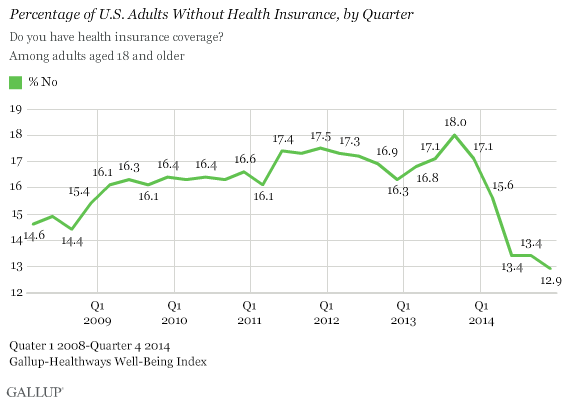
\includegraphics[width=3in]{graph-healthcare-percentage.png}
		\caption{Uninsured Rate Sank to 12.9\% in Q4 of last year}
		\label{fig:uninsured-percent}
	\end{figure}
	\subsection{Failures}
	Despite these successes. Support for the newly created Affordable Care Act program was shaken by the abysmal roll out. In the first week, the newly launched site received 20 Million visits, and yet of the 3.7 million Americans who attempted to register to shop the newly created marketplace, only about one third were successful. Leaving at least 2 million Americans to wait patiently while the issues were resolved. \cite{hc_informationweek}  make matters worse, there was plenty of blameshifting after the issues were found. 
	\subsection{Cause of Failures}

\section{DIA Baggage System}
	The DIA Baggage System is the, now dismantled, automated baggage system for the Denver International Airport. It is widely considered to be a massive flop, although after it was dismantled, its replacement did not do much better, with entire loads of luggage at times missing their respective flights completely. \cite{dia_denverpost} 
	\subsection{Successes}
		The only successes that could be cited of the DIA Baggage System is it's revolutionary nature. It never properly accomplished its goal. It required more human intervention than its non-automated counterparts, and delayed the opening of the airport by 16 months.
	\subsection{Failures}
		Revisiting the failures that were just discussed, The automated baggage system never accomplished what its goals. It frequently had failures, being cited as "eating people's baggage."\cite{dia_calleam} United after dismantling the system estimates that it will net a savings of \$1 million per year in maintenance costs.\cite{dia_nbc} 
	\subsection{Cause of Failures}
		The failures within this project are well outlined in the Calleam report. It is easily apparent that the designers of the original system grossly underestimated the complexity of the problem at hand. To make matters worse, those that took up the project later continued to expand scope without regard for the safeguards and redundancies that should have been added to deal with the extra load. So the final system was left with no backups and no fail-overs for the main junctures. This meant that the system was destined to fail the moment that a single failure occurred. \cite{dia_calleam}
\section{Comparison of systems}

\section{Conclusions}

\bibliographystyle{IEEEtran}
\bibliography{references}
\end{document}